%%%%%%%%%%%%%%%%%%%%%%%%%%%%%%%%%%%%%%%%%%%%%%%%%%%%%%%%%%%%%%%%%%%%%%%%%%%%%%%%%
%%%%%                             DATA SAMPLE                                %%%%
%%%%%%%%%%%%%%%%%%%%%%%%%%%%%%%%%%%%%%%%%%%%%%%%%%%%%%%%%%%%%%%%%%%%%%%%%%%%%%%%%

In this section we describe the construction of our data. First, we explain in detail
what our sources of data are and the steps we take to put them together in a zipcode
monthly date panel. Later, we explore how the sample of zipcodes available in Zillow, 
our source for rents data, compares to the U.S. sample of zipcodes. We conduct our 
main analysis on a balanced panel of zipcodes which construction we describe as well.

%%%%%%%%%%%%%%%%%%%%%%%%%%%%%%%%%%%%%%%%%%%%%%%%%%%%%%%%%%%%%%%%%%%%%%%%%%%%%%%%%
\subsection{Rents data from Zillow}

One of the main challenges to estimate the effects of any policy on the housing market
is to obtain data reliable data. In particular, rents data has been particularly scant
in the literature. Recent papers have used Small Area Fair Market Rents 
(SAFMRs) series from the US Department of Housing and Urban Development (\citeyear{hud}), 
available at the zipcode and year level \parencite{Tidemann2018, Yamagishi2019}. We, 
on the other hand, leverage newly available data from Zillow at the zipcode and month 
level. We think that the high frequency of the Zillow data is an advantage, since it 
allows us to identify the effect of MW changes right in the month they are enacted.

Zillow is the leader online real estate and rental platform in the U.S., hosting more 
than 110 million homes and 170 million unique monthly users in 2019 
\parencite{ZillowFacts}. Zillow provides the median rental and sale price (both 
total and per square foot) among homes listed on the platform in a given period. Time 
series are provided for different house types and at several geographic and time 
aggregation levels \parencite{ZillowData}.\footnote{See \textcite{ZillowData} for 
	more details on the data shared by Zillow. The availability of different time 
	series changed over time, so not all series used for the analysis might be still 
	available to download.} 
We collect the USPS zipcode level monthly time series. The timespan of the data 
varies at the zipcode level. As explained below, we construct a balanced panel to
address the changing composition of the sample.

Clearly, even within a single zipcode, there could be great heterogeneity in terms of 
house sizes and types, threatening the validity our estimations. In an effort to 
minimize price variation arising from houses' characteristics, we focus our main 
analysis on one housing category: \textit{single family, condominium and cooperative} houses
(SFCC). This is by far the series with the largest number of non-missing zipcodes, as 
it covers the most common U.S. rental house types. In fact, roughly a third of the 
nation's 47.2 million rental units in 2018 fit the category single-family homes, with 
the remaining 43 percent made up from buildings with 5 or more units 
\parencite{fernald2020americas}. We then focus on \textit{per square foot} variables 
for our analysis to further minimize variation arising from confounding characteristics
of the housing units. As a result, we choose the median rental per square foot in the 
SFCC category among units listed in the platform for a given zipcode and month as 
the main outcome variable. 

The Zillow data has several limitations. The first one is that we do not observe the 
underlying number of houses listed for rent in a given month. Changes in the inventory 
therefore introduce additional variation in the reported median rental price. We do 
observe the number of houses listed \textit{for sale}, which we use as a proxy for this 
variable in robustness analysis. A second limitation is that the sample of zipcodes 
available for rent is dictated by the penetration of Zillow in the housing market in the 
area. As a result, we observe a selected sample of typically urban zipcodes. We describe 
our sample in more detail later in this section.

To ensure that our data correctly captures the price evolution of the US rental market, 
we compare Zillow's median rental price with 5 SAFMRs series for houses with different 
number of bedrooms (0, 1, 2, 3, and 4 or more). SAFMRs are 
calculated for zipcodes within metropolitan areas at a yearly level, and generally correspond to 
the 40th percentile of the rent distribution for that zipcode.\footnote{For more 
	information on how SAFMRs are calculated, see \textcite[][page 41641]{hudPreamble}.} 
The yearly time series correlation between Zillow SFCC and all of the SAMFRs series is 
consistently above 90 percent. \autoref{fig:trend_zillow_safmrwgt} in the appendix 
compares the time series variation of the Zillow SFCC series and a weighted average of 
the SAFMR series for different number of bedrooms.\footnote{
	\label{foot:zillow_time_series}
	To compute the weighted SAMFR series we proceed as follows. First, we compute the 
	national yearly average for both the Zillow SFCC and the 5 	SAFMR series. Then, for 
	each of the latter we compute the U.S. share of single family, condo, and cooperative 
	houses with that number of bedrooms using the \textit{American Housing Survey} (AHS). 
	To ensure comparability, we only use the estimated count for rental houses in this 
	step. (Additionally, AHS data is available only for years 2011, 2013, 2015, 2017, and 
	2019. We therefore fill missing years with previous year's share.) Finally, we weight 
	SAFMR series using the aforementioned shares.} 
The Zillow rent data is always higher in levels. Part of this difference is intuitively 
related to the fact that Zillow reports median rent prices while SAFMRs are based on the 
40th percentile of the rent distribution. The two series however show similar trends, 
confirming that Zillow fairly captures the overall dynamics of the U.S. rental 
market.

%%%%%%%%%%%%%%%%%%%%%%%%%%%%%%%%%%%%%%%%%%%%%%%%%%%%%%%%%%%%%%%%%%%%%%%%%%%%%%%%%
\subsection{The statutory and experienced minimum wage}\label{sec:mw_construction}

Our main explanatory variable is the minimum wage. We collect data on federal, state, 
county, and city level MWs from \textcite{VaghulZipperer2016}. We complement their data,
which runs up to mid-2016, with MW data for the years 2016 to 2019 from 
\textcite{BerkeleyLaborCenter}. Because  we are interested in studying rental dynamics at 
the zipcode level using Zillow, we assign a MW to zipcodes by taking the following steps.
First, we map each zipcode to a metropolitan statistical area or rural town using HUD 
crosswalks \parencite{hudCrosswalks}. Given that zipcodes can cross county borders, we use 
number of housing units from the 2010 census and geographic codes to map each zipcode to 
a unique county by assigning it to the one with the highest share of houses from that 
zipcode. We also map each zipcode to a county and state analogously. After this process 
we are able to assign a unique state and local level MW to each zipcode. We define the 
\textit{statutory} MW variable as the maximum between the required by the federal, state, 
county, and city levels.\footnote{Some states and municipalities issue different MW levels 
	for small businesses (usually identified by having less than 25 employees). In these cases, 
	we select the general MW level as the prevalent one. In addition, there may be different (lower) MW
levels for tipped employees. We do not account for that because employers are required to make up
for the difference between tipped MW plus tips and actual MW(\href{https://www.dol.gov/general/topic/wages
	/wagestips}{\texttt{https://www.dol.gov/general/topic/wages/wagestips}}).}
As a result, we only use MW changes that are binding, meaning that they actually impact 
that maximum. 

When restricting to the sample of zipcodes available in Zillow, our data collects 18,689 MW %is this from unbalanced panel? because in balanced we have 5283
changes at the zipcode-month level. These, in turn, arise from 151 state-level and 182 
county- and city-level changes. 
%% See analysis/sumstats
\autoref{fig:d_ln_mw_dist} shows the distribution of positive increases in our 
statutory MW variable among all zipcodes available in the Zillow data.\footnote{There
	are a few cases of decrease in the MW arising from judicial decisions overthrowing 
	local MW ordinances.}
Panel (a) shows the distribution of intensity of our MW changes. The average percent 
change among Zillow zipcodes is 5.5\%. %% From unbalanced panel in derived_large
However, we observe a decent amount of large increases. Our estimation strategy will
exploit the intensity of MW changes. On the other hand, panel (b) shows the timing of 
those MW changes between 2010 and 2019. Most changes take place in either January or
July, and the majority of them take place later in the panel.

\begin{figure}[h!]
	\centering
	\caption{Distribution of Minimum Wage changes}
	\label{fig:d_ln_mw_dist}
	\begin{subfigure}{.49\textwidth}
		\caption{Intensity}
		\includegraphics[width = \textwidth]
			{../../analysis/descriptive/output/pct_ch_mw_dist.eps}
	\end{subfigure}
	\begin{subfigure}{.49\textwidth}
		\caption{Timing}
		\includegraphics[width = \textwidth]
			{../../analysis/descriptive/output/pct_ch_mw_date_dist.eps}
	\end{subfigure}
	\begin{minipage}{\textwidth} \footnotesize
		\textit{Notes:} The histograms show the distribution of positive MW changes 
		in the full sample of zipcodes available in the zillow data. Panel (a) reports 
		the intensity of the changes in percentage terms. Panel B plots the distribution 
		across time of such changes. 
	\end{minipage}
\end{figure}

We construct an alternative measure to capture the effects of MW policies: the 
\textit{experienced} MW. The goal of this measure is to account for the fact that work 
location differs from residence. The MW that matters for a given local rental market 
is the one experienced by the people living in it, and so by tracking where people in 
each zipcode work we can get a better sense of what is the relevant MW there.

To construct this measure we need to know, for each zipcode, where workers residing in that 
zipcode work. We obtain this information from the 2017 Longitudinal Employer-Household 
Dynamics Origin-Destination Employment Statistics (LODES). In particular, we collect an 
origin-destination matrix mapping jobs from residence to workplace locations. The data 
comes at the block group level. We aggregate that to construct a zipcode residence-workplace
matrix where we observe the number of workers for each residence-workplace zipcode pair.

We then use the zipcode residence-workplace matrix to build exposure weights. 
Denote zipcodes by $i$ and monthly dates by $t$. Let 
$\mathds{Z}_i$ be the set of zipcodes in which $i$'s residents work (including $i$). 
We construct the set of weights $\{\omega_{iz}\}_{z \in \mathds{Z}_i}$ as $$\omega_{iz} = 
\frac{N_{iz}}{N_i} , $$ where $N_{iz}$ is the number of workers who reside 
in zipcode $i$ and work in $z$, and $N_i$ is the total working population of zipcode $i$.\footnote{The 
	LODES data additionally provides the number of workers 29 years old and younger, and the 
	number of workers earning less than $\$1,251$/month for each residence-workplace zipcode place too.
	We additionally compute weights based on both these sub-groups, but the experienced MW 
measures obtained are all highly correlated among each other ($\rho>0.99$ for every pair).} We
finally define the experienced minimum wage measure as

\begin{equation}
	\underline{w}^{\text{exp}}_{it} = \sum_{z \in \mathds{Z}_i} \omega_{iz} \underline{w}_{zt} \ . 
\end{equation}

The experienced MW of a zipcode is based on the minimum wages binding in other zipcodes 
where its residents work. An increase in a city, for example, may not have an impact in 
the local rental market if most residents are not minimum wage workers. It will, however, 
affect neighboring zipcodes where MW workers reside. We will use this insight in our 
analysis. See \autoref{sec:experienced_mw} for more details on this measure.

%%%%%%%%%%%%%%%%%%%%%%%%%%%%%%%%%%%%%%%%%%%%%%%%%%%%%%%%%%%%%%%%%%%%%%%%%%%%%%%%%
\subsection{Other data sources}\label{sec:data/other_data}

We collect socio-demographic information from the 2010 Census and the 5-years 2008-2012 
American Community Survey (ACS). The data is originally obtained at the Census tract 
level and mapped into USPS zipcodes using HUD crosswalks \parencite{hudCrosswalks}. We 
assign to each zipcode the following characteristics: population, number of housing units, 
median income, black population, number of unemployed, and number of college students. We 
use this information to classify zipcodes into, for example, high or low median income to 
then perform heterogeneity analysis.

To proxy for local economic activity we collect data from the Quarterly Census of 
Employment and Wages (QCEW) at the county-quarter and county-month level for each main 
industrial division.\footnote{The QCEW covers the following industrial aggregates: 
	``Agriculture, Forestry, and Fishing'', ``Mining'', ``Construction'', ``Manufacturing'', 
	``Transportation and Public Utilities'', ``Wholesale Trade'', ``Retail Trade'',
	``Financial activities'' (including insurance and real state), ``Services'', and 
	``Public Administration''.}
For each county-quarter-industry cell we observe the number of establishments and the 
average weekly wage. For each county-month-industry cell we additionally observe the number 
of employed people. We merge this data onto our zipcode-month panel based by county and 
quarterly date.

%We add data from the \textit{Building Permit Survey} (BPS) at the county-month level to 
%account for time-varying shocks in the housing market. The BPS provides building permit 
%statistics on new privately-owned residential construction disaggregated by house type. 
%Lacking information on condos and cooperative houses, we only add the number of new units 
%and the permits valuation for single family houses to each zipcode-month observation based 
%on the county and month they belong.

Finally, we use the LODES data to proxy for MW workers' residence and workplace location. 
Beyond the origin-destination matrices, the LODES data provides block-level information on 
jobs by residence area (RAC) and workplace area (WAC) characteristics. These include jobs 
for various types of workers.\footnote{LODES RAC and WAC datasets provide workers' breakdown 
	for the following characteristics: age (<29, 30-54, 55>); workers' earnings(<\$1,251/mo., \$1,251/mo.-
	\$3,333/mo., >\$3,333/mo.); NAICS(11, 21, 22, 23, 31-33, 42, 44-45, 48-49, 51, 52, 52, 54, 55, 56, 
	61, 62, 71, 72, 81, 92); race (White alone, Black or African American alone, American Indian or Alaskan 
	Native alone, Asian alone, Native Hawaiian alone, two or more race groups, not Hispanic or Latino, 
	Hispanic or Latino); educational attainment(less than high school, high school or equivalent, some 
	college or associate, bachelor's degree or advanced degree); sex (male, female).} 
We use RAC and WAC datasets to ``locate" workers likely 
to earn MW by looking at the state-level distribution of such type of workers: we build, for 
each zipcode in the sample, the share (out of the state total) of workers under 30 years 
old earning less than \$1,251 
that either \textit{live} or \textit{work} there. We take 
these data as time-invariant characteristics of our zipcodes.

\begin{table}[h!]
	\caption{Descriptive statistics of different sets of zipcodes}
	\centering
	\label{tab:desc_stats}    
	
% Table created by stargazer v.5.2.2 by Marek Hlavac, Harvard University. E-mail: hlavac at fas.harvard.edu
% Date and time: Sun, Nov 08, 2020 - 3:45:47 PM
\begin{tabular}{@{\extracolsep{5pt}} ccccc} 
\\[-1.8ex]\hline 
\hline \\[-1.8ex] 
 & U.S. & Top 100 CBSA & Full Panel & Est. Panel \\ 
\hline \\[-1.8ex] 
Population (millions) (2010) & $311.18$ & $189.71$ & $110.17$ & $50.62$ \\ 
Population as share of U.S. & $1$ & $0.61$ & $0.35$ & $0.16$ \\ 
Housing Units (millions) (2010) & $132.83$ & $78.74$ & $46.72$ & $21.32$ \\ 
Housing Units as share of U.S. & $1$ & $0.59$ & $0.35$ & $0.16$ \\ 
Urban Share (2010) & $0.46$ & $0.75$ & $0.96$ & $0.97$ \\ 
College Share (2010) & $0.46$ & $0.75$ & $0.96$ & $0.97$ \\ 
African-American Share (2010) & $0.46$ & $0.75$ & $0.96$ & $0.97$ \\ 
Hispanic Share (2010) & $0.10$ & $0.14$ & $0.17$ & $0.19$ \\ 
Elder Share (2010) & $0.15$ & $0.13$ & $0.12$ & $0.11$ \\ 
Poor Share (2010) & $0.46$ & $0.75$ & $0.96$ & $0.97$ \\ 
Unemployed Share (2010) & $0.09$ & $0.09$ & $0.09$ & $0.09$ \\ 
Mean HH income (2010) & $52,492.56$ & $62,773.64$ & $65,475.16$ & $66,919.72$ \\ 
Rent House Share (2010) & $0.29$ & $0.35$ & $0.38$ & $0.38$ \\ 
Work in same county share (2010) & $0.70$ & $0.68$ & $0.76$ & $0.76$ \\ 
Unique zipcodes & $38,893$ & $14,583$ & $3,315$ & $1,305$ \\ 
Share of state events & $$ & $$ & $0.03$ & $0.03$ \\ 
Share of county events & $$ & $$ & $0.001$ & $0.001$ \\ 
Share of  localevents & $$ & $$ & $0.003$ & $0.0005$ \\ 
Mean SFCC psqft rent & $$ & $$ & $1.30$ & $1.27$ \\ 
Unique zipcodes SFCC psqft rent & $$ & $$ & $3,316$ & $1,143$ \\ 
\hline \\[-1.8ex] 
\end{tabular} 

	\begin{minipage}{0.95\textwidth} \footnotesize
		\vspace{3mm} 
		\textit{Notes}: The table shows characteristics of four sets of US postal service 
		zipcodes. Column 1 reports demographic statistics for the universe of USPS zipcode we 
		were able to map. Column 2 shows the same statistics for for the top 100 Core-Based 
		Statistical Areas (CBSA). Column 3 shows the characteristics of the set of zipcodes 
		available in the Zillow data. Finally, column 4 shows the restricted balanced sample 
		we use as baseline in our empirical analysis. All demographic information comes from 
		the 2010 Census and the 5-years 2008-2012 ACS.
	\end{minipage}
\end{table}


%%%%%%%%%%%%%%%%%%%%%%%%%%%%%%%%%%%%%%%%%%%%%%%%%%%%%%%%%%%%%%%%%%%%%%%%%%%%%%%%%
\subsection{The resulting panel}

Using the data described above we put together a panel dataset at the zipcode and monthly 
date levels from January 2010 to December 2019. Given that zipcodes enter the Zillow data 
progressively over time affecting the composition of the sample, we construct our baseline 
\textit{estimating panel} by keeping in the sample those zipcodes with valid rents data as 
of July 2015. This panel contains 5,302 MW increases, which arise from 124 state changes 
and 99 county and local level changes.
%% See analysis/sumstats

We stress the fact that our data does not cover the full sample of zipcodes, but rather a
selected sample. \autoref{fig:maps} in the appendix maps the full set of available zipcodes
in the Zillow data, together with population density. The Zillow sample seems fairly 
distributed across urban areas, although some important areas have limited coverage. 

\autoref{tab:desc_stats} further compares the Zillow sample to the population of zipcodes
along several important demographic dimensions. Columns 1 and 2 report data for the whole 
universe of US zipcodes and for the top 100 US metropolitan areas, respectively. In column 
3 we show the complete set of zipcodes in the Zillow data. Finally, column 4 shows our 
baseline estimating sample. Focusing on our prefered variable --median rent per square
foot in the SFCC category--, Zillow provides information on rents for 4,604 unique zipcodes 
that amount to 11.8 percent of the 38,893 US zipcodes and 46.7 percent of the 2010 US 
population. The average median household annual income for those zipcodes is \$65,475.2, 
almost 25 percent higher than the same figure for the average US zipcode. However, average 
income is slightly lower than the top 100 metropolitan areas. Zipcodes in the baseline 
sample are slightly richer on average. 

Zillow zipcodes have a higher share of urban population, college students, and houses for 
rent than the average US zipcode. We see this as confirmation of the fact that our data 
contains zipcodes more likely to adopt Zillow as a market for rentals early on. That said, 
our zipcodes capture an important share of urban areas in the US. In an attempt to capture 
the treatment effect for the average zipcode we conduct an estimation re-weighting our 
sample to match characteristics of the top 100 CBSA sample of zipcodes. Because our 
zipcodes are richer than the average, we expect to find a larger effect in this exercise.

Finally, \autoref{tab:estimating_panel_stats} shows some basic sample statistics of our 
baseline estimating panel. As is apparent from the table, the statutory and experienced
MW are highly correlated. We also show summary statistics of median rents in the SFCC 
category (absolute and per square foot) and average wage, employment and establishment 
count for the Financial sector. \autoref{tab:estimating_panel_stats_long} in the appendix 
shows a longer version of this table that includes more rent variables and the full set
of industries we use as controls in our regressions.

\begin{table}[h!]
	\caption{Descriptive statistics of estimating panel}
	\centering
	\label{tab:estimating_panel_stats}    
	
% Table created by stargazer v.5.2.2 by Marek Hlavac, Harvard University. E-mail: hlavac at fas.harvard.edu
% Date and time: Mon, Nov 30, 2020 - 11:59:17 AM
\begin{tabular}{@{\extracolsep{5pt}}lccccc} 
\\[-1.8ex]\hline 
\hline \\[-1.8ex] 
Statistic & \multicolumn{1}{c}{N} & \multicolumn{1}{c}{Mean} & \multicolumn{1}{c}{St. Dev.} & \multicolumn{1}{c}{Min} & \multicolumn{1}{c}{Max} \\ 
\hline \\[-1.8ex] 
Statutory MW & 156,600 & 8.08 & 1.21 & 7 & 16 \\ 
Experienced MW & 156,600 & 8.06 & 1.20 & 6.29 & 14.98 \\ 
Median rent psqft. SFCC & 113,375 & 1.27 & 0.83 & 0.47 & 7.25 \\ 
Median rent SFCC & 125,644 & 1,651.10 & 702.99 & 595.00 & 6,595.00 \\ 
Avg. wage Fin. activities & 152,334 & 1,561.78 & 965.27 & 0.00 & 9,557.00 \\ 
Employment Fin. activities & 152,334 & 59,554.22 & 75,796.09 & 0.00 & 397,839.00 \\ 
Estab. count Fin. activities & 152,334 & 5,103.83 & 5,200.06 & 31.00 & 30,405.00 \\ 
\hline \\[-1.8ex] 
\end{tabular} 

	\begin{minipage}{0.95\textwidth} \footnotesize
		\vspace{3mm} 
		\textit{Notes}: The table shows summary statistics of our baseline estimating panel.
		Variables included are the statutory and experienced MW, constructed as explained in
		\autoref{sec:mw_construction}; the average of median monthly rents per square foot 
		and total in the SFCC category, taken directly from Zillow; and average weekly wage, 
		employment and establishment count in the Financial Sector from the QCEW.
	\end{minipage}
\end{table}
